\header{
    \section{La digue du cul} \label{la-digue-du-cul}
    %
    
    \insertComment{Présence à Montaigu de contingents de soldats venant de Nantes et allant à Rochefort; daté d'avant 1586 (démentelment de la digue de Montaigue par Henri III).}{}
}
%
\enluminure{3}{\href{https://www.youtube.com/watch?v=4QQlvTUD-us}{L}}{a digue} du cul en revenant de Nantes ~~~~\bissimple
\\De Nantes à Montaigu la digue la digue
\\De Nantes à Montaigu la digue du cul !
%\\\\\textbf{Refrain :}
%\\Lève la jambe, voilà qu'ça rentre
%\\Lève la cuisse, la cuise, la cuisse
%\\Voilà qu'ça glisse
%\\Lève la jambe, voilà qu'ça rentre
%\\Lève la cuisse, la cuise, la cuisse
%\\Voilà qu'ça glisse
%\\Oh ! Hisse
\\\\La digue du cul sur la route de Nantes  ~\bissimple
\\De Nantes à Montaigu la digue la digue
\\De Nantes à Montaigu la digue du cul !
\\\\La digue du cul je rencontre une belle ~\bissimple
\\Qui dormait le cul nu la digue la digue
\\Qui dormait le cul nu la digue du cul !
\\\\La digue du cul je bande mon arbalète  ~~~~~~\bissimple
\\Et lui fous droit dans l'cul la digue la digue
\\Et lui fous droit dans l'cul la digue du cul !
\\\\La digue du cul la belle se réveille  ~~~~~~~~~~~~\bissimple
\\Et s'dit j'ai l'diable au cul la digue la digue
\\Et s'dit j'ai l'diable au cul la digue du cul !
\\\\La digue du cul non ce n'est pas le diable  ~\bissimple
\\Mais un beau dard poilu la digue la digue
\\Mais un beau dard poilu la digue du cul !
\breakpage
La digue du cul qui bande et qui décharge  ~\bissimple
\\Et qui t'en fout plein l'cul la digue la digue
\\Et qui t'en fout plein l'cul la digue du cul !
\\\\La digue du cul si ce n'est pas le diable  ~~\bissimple
\\Refous-moi le dans l'cul la digue la digue
\\Refous-moi le dans l'cul la digue du cul !
\\\\La digue du cul s'il y'est bien qu'il y reste ~\bissimple
\\Et qu'il n'en sorte plus la digue la digue
\\Et qu'il n'en sorte plus la digue du cul !
\bigskip
\bigskip
\bigskip
\begin{center}
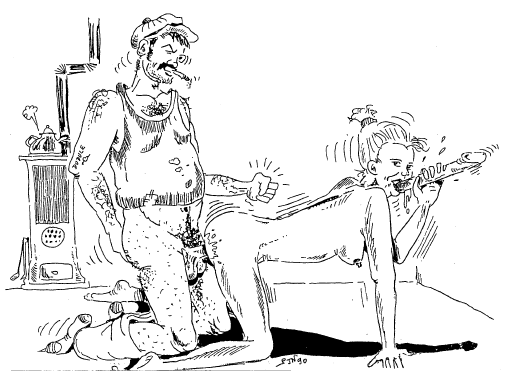
\includegraphics[width=1\textwidth]{images/image4.PNG}
\end{center}

\breakpage